\chapter{Marco teórico}
\label{capitulo1}
\lhead{Capítulo 2. \emph{Marco teórico}}


En el cap\'itulo se describir\'an algunos conceptos importantes para comprender la implementaci\'on del sistema  en el que se basa el presente trabajo. Dichos conceptos son: \textit{IDS, el protocolo HTTP, URI , autom\'atas de estados finitos, autom\'atas probabilísticos, modelo de Markov,SSM y Bro}.

En l\'ineas generales, se tiene como prop\'osito explicar el funcionamiento de un \textit{IDS} basado en anomalías que haga uso del sistema \textit{SSM} y del lenguaje de scripting de la herramienta \textit{BRO}.

Este sistema analiza los \textit{URI} de las peticiones tipo GET o HEAD del protocolo \textit{HTTP}, haciendo uso de la t\'ecnica \textit{SSM}. Esta t\'ecnica, a su vez hace uso de \textit{autómatas de estados finitos probabilísticos} y del \textit{modelo de Markov} para determinar si las peticiones realizadas a un servidor \textit{HTTP} son posibles ataques o no.
% De qué va a tratar el capítulo
% El capítulo 1 suele ser el marco teórico.

\section{Protocolo HTTP}

El protocolo HTTP, (``Hypertext Transfer Protocol'') es un protocolo de la capa de aplicación que se encuentra en el corazón de la Web. Se define en [RFC 1945] y [RFC 2616]. HTTP esta implementado en dos programas: un programa cliente y un programa servidor. El programa cliente y el programa servidor se ejecutan en diferentes sistemas y se comunican entre si intercambiando mensajes HTTP. HTTP por su parte, define la estructura de dichos mensajes y como se realiza el intercambio de los mismos. \cite{httpKross}

El protocolo HTTP, es un protocolo simple de petición-respuesta que funciona normalmente sobre la capa de transporte TCP. La idea general de la interacción entre el cliente y el servidor se muestra en la figura \ref{fig:httpPeticionRespuesta}. 

\begin{figure}[tb]
\begin{center}
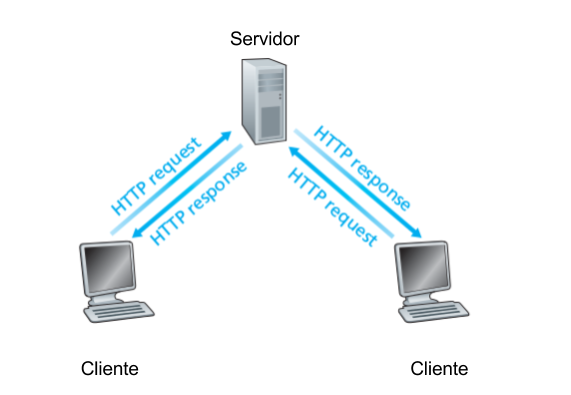
\includegraphics[width=3in]{HTTP.png}
\caption{Petición-respuesta.\cite{httpKross}}
\label{fig:httpPeticionRespuesta}
\end{center}
\end{figure}

En el protocolo HTTP, el cliente inicia la conexión TCP con el servidor. Una vez establecida la conexión, ambos podrán enviar y recibir mensajes de petición y respuesta. La información que se transfiere mediante este protocolo pueden ser archivos de texto plano, hipertexto, audio, imágenes o cualquier información accesible por Internet.

Es importante tener en cuenta que el servidor envía los archivos solicitados a los clientes sin almacenar información del estado de los mismo, es decir, el servidor no almacena información de sus clientes. Debido a esto se dice que HTTP es un protocolo sin estado.\cite{httpKross}

Por otra parte, los mensajes de petición y respuesta del protocolo HTTP poseen una estructura general como la que se muestra en la figura \ref{fig:httpMensaje}.

\begin{figure}[tb]
\begin{center}
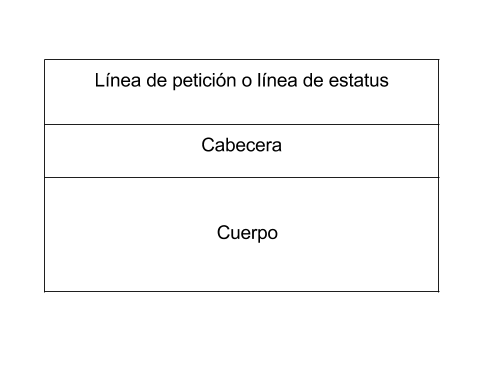
\includegraphics[width=3in]{mensajeHTTP.png}
\caption{Mensaje HTTP.\cite{httpKross}}
\label{fig:httpMensaje}
\end{center}
\end{figure}

La linea de petición en los mensajes HTTP, presenta tres partes separadas por espacios:

\begin{enumerate}
\item El método.
\item El identificador del recurso solicitado (URI).
\item La version del protocolo HTTP.
\end{enumerate}

El método es un parámetro que indica lo que actualmente se esta solicitando por el mensaje. 
Los m\'etodos GET, HEAD y POST son los más utilizados en las comunicaciones del protocolo HTTP. 

\begin{itemize}
\item GET se encarga de hacer solicitudes de recursos al programa servidor HTTP.
\item HEAD solicita recursos de la misma forma en la que lo hace el método GET con la \'unica diferencia de que la solicitud solo ser\'a respondida con la cabecera del recurso, excluyendo el cuerpo del mismo.
\item POST solicita que el recurso de destino  procese la informaci\'on que viene incluida en la solicitud realizada
\end{itemize}

Para el presente trabajo la sintaxis de los URI y los mensajes de petición de tipo GET resultan de importante relevancia.

\section{URI} \label{URIsection}

Un URI es una serie de caracteres que identifican un recurso en la red. Este posee una sintaxis específica que está conformada por diferentes segmentos de caracteres: el esquema, la autoridad, la ruta, el ``query'' y el ``fragment''.

En la figura \ref{fig:URI}, se muestra, en un ejemplo de los componentes que forman un URI.

\begin{figure}[H]
\begin{center}
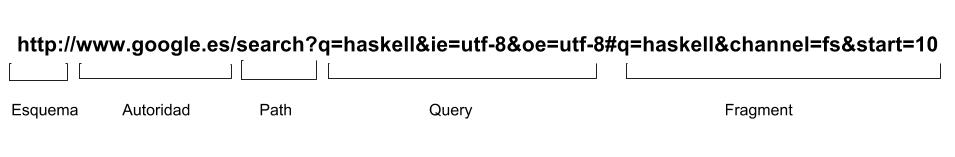
\includegraphics[width=3in]{./URI.jpg}
\caption{URI.}
\label{fig:URI}
\end{center}
\end{figure}

A continuaci\'on se describe de manera breve cada uno de los componentes que pueden conformar un URI.

\begin{itemize}

\item Esquema:

El esquema identifica el protocolo. En el caso del presente trabajo, los URIs utilizaran únicamente el protocolo http o https.


\item Autoridad:

Este componente del URI posee información del ``host'' del URI, el cual viene representado bien sea por un IPv4 o un nombre de dominio, seguido de un número de puerto (opcional).
   
\item ``Path'':
La ruta de un URI es un conjunto de segmentos organizados de manera jerárquica que contienen información sobre la ubicación de los recursos a solicitar.

\item ``Query'':

El ``query'' de un URI es un segmento de información no jerarquizada, cuyo símbolo de inicio es el signo de interrogación (?). Por lo general, el ``query'' está conformado por una dupla ``atributo=valor'' que junto con la ruta identifican el recurso que se desea solicitar. A diferencia de la ruta, la información aquí contenida debe ser procesada por el servidor al que se le está solicitando el recurso. 

\item ``Fragment'':

En un URI, el ``fragment'' corresponde a la dirección de un segundo recurso dentro del primer recurso identificado por la ruta y el ``query''. Esta cadena de caracteres esta precedida por el símbolo de un numeral (\#).

\end{itemize}

En un URI, tanto el esquema como la ruta son segmentos que deben existir de manera obligatoria. Si la ruta es un carácter vac\'io, se asumir\'a que la misma es ``/''. El resto de los segmentos son opcionales.

\section{Detector de intrusiones (IDS)}
Un detector de intrusiones (IDS del inglés "Intrusion-detection system" ) es un sistema que se encarga de procesar la información entrante de un sistema a proteger con la intención de detectar actividades maliciosas y lanzar alertas para activar el proceso de auditoría por parte de los administradores de sistema \cite{IDS}

Los IDS suelen clasificados en: IDS basados en firmas o 		IDS 	basados en anomalías. 

Los IDS basados en firmas, utilizan una base de datos de ataques conocidos y vulnerabilidades del sistema los cuales son utilizados para realizar comparaciones con los patrones seguidos por las actividades detectadas. Si se detecta similitud con alguno de los patrones de la base de datos, se activará una alarma para indicar que un ataque esta siendo perpetuado.

La eficacia de los detectores de intrusiones basados en firmas es muy buena, sin embargo, su buen funcionamiento depende completamente de la constante actualización de la base de datos de ataques.

Por otra parte, los IDS basados en anomalía detectan los ataques de manera diferente. En este tipo de IDS los ataques son detectados a partir de la observación de comportamientos, bien sea del sistema, o de los usuarios. 

El modo de funcionamiento de un IDS basado en anomalía se basa en: recolectar la información de las actividades detectadas y comparar dicha información con un modelo de normalidad del sistema que ha sido previamente construido. El modelo de normalidad se construye a partir de comportamientos previamente observado en el sistema y que son catalogados como "normales". Si existe una incongruencia entre la información entrante y el modelo de normalidad, entonces se generará una alarma.

No obstante, uno de los problemas de este tipo de detector de intrusiones es la alta tasa de falsos positivos que puede llegar a tener. Esto se debe, a que los modelos, por lo general, no contienen todos los comportamientos normales de un sistema en su totalidad. Esto, a su vez provoca que existan eventos libres de ataques que sean catalogados como una amenaza. Tambi\'en está el hecho de que es muy posible que con el pasar del tiempo, el comportamiento del sistema a proteger vaya cambiando, lo cual implicar\'ia que, si no se hace una constante revis\'on y reentrenamiento del modelo de normalidad el mismo quedar\'a obsoleto y los eventos entrante ser\'an mal catalogados por el IDS. El problema de realizar entrenamientos constantes para actualizar un modelo de normalidad es que se crearán brechas de tiempo en donde el sistema ser\'a muy vulnerable a ataques ya que en lugar de estar funcionando el módulo para detección, estar\'a funcionando el módulo para entrenar el modelo de normalidad. Por lo tanto, si un ataque es perpetrado durante ese periodo de tiempo, el mismo quedar\'a grabado en el modelo de normalidad como un comportamiento normal del sistema.

También existen los IDS híbridos cuyo funcionamiento mezcla el funcionamiento de los detectores de intrusiones basados en firmas y los basados en anomalía, es decir, este tipo de  IDS suelen contar con una base de datos de firmas y también con un modelo de normalidad.

\section{Autómatas de estados finitos}

Un autómata es un modelo abstracto de un ordenador digital \cite{automata}. Una manera de definirlo de forma gráfica es como se muestra en la figura \ref{fig:automata}.

\begin{figure}[H]
\begin{center}
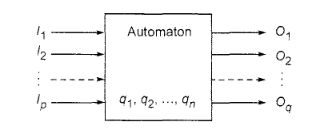
\includegraphics[width=3in]{automata.png}
\caption{Autómata.\cite{automata2}}
\label{fig:automata}
\end{center}
\end{figure}

donde \cite{automata2}:

\begin{itemize}
\item  $I_{1}, I_{2},..., I_{n}$ es el "input" del autómata  que es introducido en cada instante de tiempo $t_{1}, t_{2},..., t_{n}$.

\item $O_{1}, O_{2},..., O_{n}$ es la salida del autómata.

\item $q_{1}, q_{2},..., q_{n}$ son los estado en los que puede estar el autómata en cualquier instante de tiempo.
\end{itemize}

Dentro de los autómatas existe la familia de los autómatas de estado finito. Un autómata de estado de autómata finito se puede definir formalmente como una quíntupla \cite{automataFinito}:.

\begin{equation}
M = (Q,\Sigma,\delta,q,F)
\end{equation}

donde:

\begin{itemize}

\item Q es un conjunto finito de estados.

\item  $\Sigma$ es un conjunto finito, llamado alfabeto. Los elementos de $\Sigma$ se llaman símbolos.

\item $\delta$ es una función de transición, tal que $ Q x \Sigma \leftarrow Q$
 
\item  q  es un elemento perteneciente a Q llamado estado inicial.

\item F es un subconjunto de Q y representa el conjunto de estados finales.

\end{itemize}

Los autómatas finitos se clasifican en autómatas finitos deterministas (DFA, del inglés "Deterministic Finite Automata") y no-deterministas (NFA, del inglés "Nondeterministic Finite Automata").

Los autómatas finitos deterministas se definen teóricamente de la misma manera en la que se definen los autómatas finitos. Sin embargo, se debe cumplir que por cada estado $"s"$ y símbolo de entrada $"a"$ debe existir un único estado al que se puede hacer una transición. Esto quiere decir que la función de transición $\delta$ de los autómatas finitos deben retornar un solo elemento.

Por otra parte, los autómatas finitos no-deterministas al igual que los autómatas finitos deterministas se definen teóricamente de la misma forma que los autómatas finitos. No obstante, la función de transición $\delta$ de estos autómatas puede retornar un conjunto de elementos, es decir, por cada estado $"s"$ y símbolo de entrada $"a"$ pueden existir varios estados al los que se puede hacer una transición.

Tanto los autómatas finitos deterministas como los no deterministas se puede representar a tráves de un grafo. En donde los estados serian representados a tráves de los nodos y las aristas representarían las funciones de transición. 

Un ejemplo de un NFA representado a tráves de un grafo se presenta en la figura \ref{fig:NFA}.

\begin{figure}[H]
\begin{center}
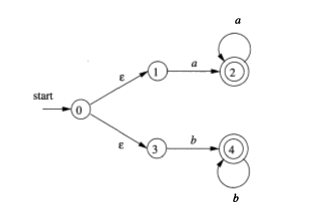
\includegraphics[width=3in]{NFA.png}
\caption{Autómata no-determinista.\cite{automataFinito}}
\label{fig:NFA}
\end{center}
\end{figure}

En la figura \ref{fig:DFA} se muestra la representación de un DFA haciendo uso de un grafo.

\begin{figure}[H]
\begin{center}
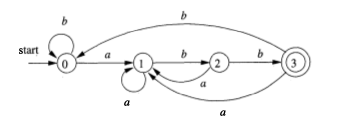
\includegraphics[width=3in]{DFA.png}
\caption{Autómata determinista.\cite{automataFinito}}
\label{fig:DFA}
\end{center}
\end{figure}

Los autómatas deterministas permitirían determinar, dado un autómata asociado a un protocolo, si una secuencia de mensajes intercambiados puede ser decodificada mediante dicho autómata. Esto es, si la secuencia de mensajes corresponde a la especificación del protocolo y, por lo tanto, es gramaticalmente correcta. No obstante, una parte importante de los ataques son estructuralmente correctos de acuerdo al protocolo, es decir, siguen la gramática \cite{tesisMexico}.

Sin embargo, los autómatas no deterministas permitirán discriminar ataques cuya estructura sintáctica sea correcta porque permiten incorporar información relacionada con la semántica o el contexto .

Un tipo de autómata no determinista de especial interés para los objetivos del presente trabajo son los autómatas de estado finitos probabilístico [Brookshear, 1989]. En estos se consideran probabilidades asociadas a los estados y/o a los símbolos de forma que se atribuye una naturaleza probabilística tanto a la secuencia de estados que sigue el sistema como a la de los símbolos observados.


\section{Modelo de Markov}

En un proceso de Markov un evento en un tiempo determinado, depende de los procesos inmediatos anteriores a este \cite{markov}. Un modelo de Markov discreto, por otra parte, consiste en un conjunto de estados y una serie de probabilidad de transición que rigen las transiciones entre estados y la producción de símbolos.

Un modelo de Markov discreto, $\lambda$, se define como un quíntupla:

\begin{equation}
\lambda = (Q,\Theta,A,B,\Pi)
\end{equation}

donde:
 
\begin{itemize}
\item Q :  Es el conjunto de N estados del modelo.
\item $\Theta$ : Es el vocabulario del modelo, es decir, son los posibles s\'imbolos o eventos observables del sistema.
\item A : Es una matriz NxN de probabilidades de transici\'on entre estados.
\begin{equation}
\begin{aligned}
A = [a_{ij}], 1\leq i \leq N  y  1\leq j \leq N.\\
a_{ij} = P(q_{t} = S_{j} | q_{t-1} = S_{i})
\end{aligned}
\end{equation}

\item B : Es una matriz NxM de probabilidades de generaci\'on u observación de los s\'imbolos .
\begin{equation}
\begin{aligned}
B = [b_{ik}], 1\leq i \leq N, 1\leq k \leq M.\\
b_{ik} = P(O_{t} = v_{k} | q_{t} = S_{i})
\end{aligned}
\end{equation}

\item $\Pi$ es el vector de probabilidades del estado inicial.
\begin{equation}
\begin{aligned}
\Pi = [\Pi_{i}], 1\leq i \leq N \\
\pi_{i} = P(q_{1} = S_{i})
\end{aligned}
\end{equation}

\end{itemize}

Un ejemplo sencillo de un modelo de Markov sería el siguiente \cite{ejemploMarkov}

S = {$s_{1}$,$s_{2}$}, donde, $s_{1} = "lluvioso"$ y $s_{2} = "soleado"$ y la matriz de transición es:

\[
 P = \begin{pmatrix}
  0.75 & 0.25  \\
  0.25 & 0.75  \\
 \end{pmatrix}
\]

Un modelo de Markov es un autómata de estados finitos no determinista que puede ser representado mediante grafos.

El ejemplo presentado con anterioridad, por lo tanto se puede graficar de la manera en la que se muestra en la figura \ref{fig:modeloMarkov}.

\begin{figure}[H]
\begin{center}
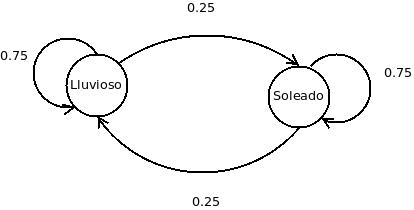
\includegraphics[width=3in]{ejemploMarkov.jpeg}
\caption{Ejemplo modelo Markov.}
\label{fig:modeloMarkov}
\end{center}
\end{figure}


\section{SSM}\label{sec:modeloSSM}

SSM o \textit{Structural Stochastic Modeling} en ingl\'es es una tecnica desarrollado por Estevez-Tapiador. A grandes rasgos, esta t\'ecnica se basa en la definición de un autómata de estados finitos estocástico capaz de evaluar la probabilidad de generación de una petición concreta. El autómata permitirá, por tanto, dada una petición, evaluar si dicha petición es legítima (corresponde al modelo) y su probabilidad. En función de la probabilidad y de un umbral se clasificaran las peticiones como normales o anormales.\cite{ssm}

Esta t\'ecnica, se basa en la teor\'ia de los modelos de Markov ya que se define un autómata de estados finitos que permite evaluar la probabilidad de generaci\'on de una petici\'on, dado un modelo previamente construido.

Por otra parte, en el presente trabajo, las peticiones que ser\'as estudiadas por dicha t\'ecnica ser\'an peticiones de tipo GET del protocolo HTTP. En concreto, de las peticiones GET el elemento a estudiar ser\'an los URIs de dichas peticiones. No obstante, se puede extender para que funcione con m\'etodos de tipo POST y HEAD. 

\begin{figure}
\begin{center}
  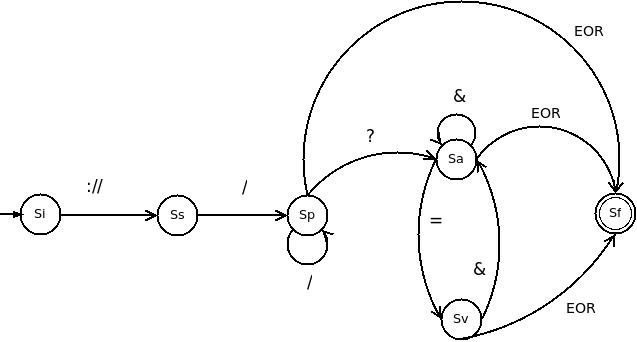
\includegraphics[width=\linewidth]{ssm.jpeg}
  \caption{Automata del modelo SSM}
  \label{fig:ssm}
\end{center}

\end{figure}

Este hecho hace que el autómata de SSM deba tomar una cierta topolog\'ia para que de esta forma se puedan reconocer los URIs de cada petici\'on. Dicha topolog\'ia se infiere a tráves de la sint\'axis de los URIs. En la figura \ref{fig:ssm} se muestra la topolog\'ia del autómata.

Las transiciones del autómata vienen dada, por las especificaciones de las sintaxis de los URIs, que est\'an descritas en el RFC 3986. Adem\'as, se puede observar en la figura \ref{fig:ssm} que el autómata tiene un estado inicial ($S_{I}$), un estado del ``host'' ($S_{S}$), un estado de segmento de ruta ($S_{P}$), un estado atributo ($S_{A}$), un estado valor ($S_{V}$), un estado final ($S_{F}$) y un estado sumidero ($S_{OOS}$) en el que se termina si el URI no es sint\'acticamente correcto.

Si una petici\'on del protocolo HTTP anexa un URI que no puede ser reconocido por el autómata descrito con anterioridad implicar\'a que el URI de dicha petici\'on no est\'a bien construido sintácticamente.

Adem\'as, existirá un vocabulario diferente para los estados $S_{S}$, $S_{P}$, $S_{A}$ y $S_{V}$. Estos vocabularios, son construidos, a partir de tomar m\'ultiples peticiones libres de ataques realizadas al servidor. 

Entonces, en resumen, lo que hace la t\'ecnica de SSM para detectar intrusiones es verificar la sintaxis del URI de las peticiones enviadas al servidor a tráves del autómata descrito con anterioridad y, al mismo tiempo, se estudia segmento por segmento del URI la probabilidad que tiene cada palabra de aparecer en un estado determinado del autómata, para as\'i verificar si el URI que viene anexado al la petici\'on es una cadena de caracteres que probabilísticamente corresponde a un petici\'on normal o no.

Teóricamente, el modelo utilizado por SSM es el siguiente \cite{tesisMexico}:

\begin{itemize}
\item Q: es el conjunto de estados ($S_{I}$,$S_{S}$,$S_{P}$,$S_{A}$,$S_{V}$,$S_{F}$,$S_{OOS}$).
\item $\theta$: es el conjunto de s\'imbolos observables que se encuentran en el vocabulario de cada estado.
\item A: es la matriz de probabilidad de transiciones entre estados
\item B: es un conjunto de vectores que contiene la probabilidad de las palabras observadas en cada estado. ($B_{I}$,$B_{S}$,$B_{P}$,$B_{A}$,$B_{V}$,$B_{F}$,$B_{OOS}$).
\item $\Pi$: es el vector de probabilidades iniciales, cuyos valores est\'an determinados por la topolog\'ia del modelo. 
\end{itemize}

\subsection*{Evaluación}
\label{subsec:exprIndice}

Dado un conjuntos de observaciones $0 = o1,o2,...,oT$. Cada una pertenecientes a los estados $Q = q1,q2,..,qT$. En principio, se puede realizar la evaluación de un URI, dado un modelo $\lambda$,  calculando la probabilidad del conjunto completo de observaciones O del modelo $\lambda$ siguiendo el patrón de la secuencia de estados Q. Es decir:

\begin{equation}
P(O|\lambda,Q) = \pi_{q1}b_{q1o1}\prod_{t=1}^{T-1}a_{q_{t}q_{t+1}}b_{q_{t+1}o_{t+1}}
\end{equation}

Para evitar problemas de desbordamiento de calcula el logaritmo de la probabilidad en lugar de la probabilidad.

\begin{equation}\label{eq:Probabilidad}
log(P(O|\lambda,Q)) = log(\pi_{q1}b_{q1o1}\prod_{t=1}^{T-1}a_{q_{t}q_{t+1}}b_{q_{t+1}o_{t+1}})
\end{equation}

Si se considera que las probabilidades iniciales son cero excepto para S1 y que las probabilidades de transición son equivalentes a 1. Entonces, se tendría que la fórmula presentada en \ref{eq:Probabilidad} se podría resumir en la siguiente:

\begin{equation}
P(O|\lambda,Q) = \sum_{t=1}^{T}b_{q_{t}o_{t}}
\end{equation}

Entonces, en primera instancia se podría decir que el índice de anormalidad de un URI U, dado un modelo $\lambda$, se puede obtener de la siguiente forma:

\begin{equation}\label{eq:Probabilidad2}
N_{s} = -log(P(U|\lambda))
\end{equation}

La fórmula \ref{eq:Probabilidad2} será aplicada sólo si el URI U llega al estado final Sf, de otra manera al índice de anormalidad Ns se le será asignado $\infty$, es decir:

\begin{equation}\label{eq:Ns1}
N_{s} = 
	\begin{cases} 
      -log(P(U|\lambda)) & $si $  q_{t} = S_{f} \\
      \infty & $si $  q_{t} \neq S_{f} \\ 
   \end{cases}
\end{equation}

Como se puede observar en la fórmula \ref{eq:Ns1}, mientras menor sea la probabilidad de aparición de las observaciones, mayor será el índice de anormalidad, por esta razón, una vez calculado el índice, se podría decir que un URI U es anómalo, si el índice de anormalidad es mayor o igual a un umbral de detección $\theta$ de lo contrario se dirá que el URI no posee anomalías, esto es:

\begin{equation}\label{eq:ClaseU}
Clase(U) = 
	\begin{cases} 
      Normal & $si $  N_{s}(U) \leq \theta \\
      Anomalo & $si $  N_{s}(U) > \theta \\ 
   \end{cases}
\end{equation}


El umbral de detección es un parámetro que se calcula de forma experimental. Durante la pruebas se busca conseguir un valor $\theta$ con el cual se pueda obtener la proporción óptima entre las detecciones de anomalías correctas y los falsos positivos. 

No obstante, la fórmula presentada en el apartado \ref{eq:Ns1} posee algunos inconvenientes ya que no se estipula el caso en el que existan problemas de entrenamiento insuficiente que será presentado en la sección o que los diferentes vectores B, tengan diferente número de observaciones. El segundo caso provoca un inconveniente a la hora de realizar la evaluación ya que el acumulado de las probabilidades de los vectores B estarán ligados a la longitud de los mismos. Para solucionar dicho problema se utilizara la propuesta de Estévez [Estévez-Tapiador 2004a], en el que se establece como factor de compensación la probabilidad de observación para de esta manera obtener una probabilidad normalizada. Esta sería la siguiente expresión:

\begin{equation}\label{eq:sumB}
\varepsilon_{0} = E[B] = \frac{1}{M}\sum_{i=1}^{M}b_{i}
\end{equation}

Por otra parte, el entrenamiento insuficiente es un problema que se presenta cuando se toma una palabra durante la evaluación que no pertenezca al conjunto de palabras observadas durante el entrenamiento en el modelo. Esto puede ser debido a que la palabra es una palabra anómala o que no se entrenó lo suficiente al sistema. En este caso, la solución que se le aplicará a dicho problema será la de asignar un valor fijo de probabilidad muy baja a estos casos ( poov($S_{i}$): probabilidad fuera de vocabulario). Cada uno de los estados del modelo poseerá valores independientes de probabilidades que serán utilizados una vez se detecte este problema.

El otro caso en el que se utilizarán los valores de poov($S_{i}$), es cuando la probabilidad de una palabra que está en el vocabulario es inferior al poov($S_{i}$), es decir:


\begin{equation}\label{eq:Pqtot}
p_{qtot} = 
	\begin{cases} 
      b_{qtot} & $si $  o_{t} \in O $ y $ b_{qtot} > p_{oov}(q_{t})\\
      p_{oov} & $en otro caso$ \\ 
   \end{cases}
\end{equation}


Entonces, la nueva expresión del índice de anormalidad que toma en cuenta todas las consideraciones nombradas con anterioridad, es la siguiente:

\begin{equation}\label{eq:Ns}
N_{s} = 
	\begin{cases} 
      -Tlog(\varepsilon_{0})\sum_{t=1}^{T}log(p_{qtot}) & $si $  q_{t} = S_{f} \\
      \infty & $si $  q_{t} \neq S_{f} \\ 
   \end{cases}
\end{equation}

\subsection*{Entrenamiento}

Dada una secuencia de observaciones 0 = o1,o2,...,oT ,y  su correspondiente secuencia de estados, Q = q1,q2,...,qT.

El entrenamiento requiere de un conjunto considerable de observaciones  junto con los estados asociados a cada una de ellas.

Por lo tanto, se considerara un conjunto de entrenamiento $\omega$ de L pares de secuencias de estados

\begin{equation}
\omega = {(O^{1},Q^{1}),(O^{2},Q^{2}),...,(O^{L},Q^{L})}
\end{equation}

tal que:

\begin{equation}
\begin{aligned}
O^{i} = {o_{1}^{i},o_{1}^{i},...,o_{Ti}^{i}} \\
Q^{i} = {q_{1}^{i},q_{2}^{i},...,q_{Ti}^{i}}
\end{aligned}
\end{equation}

Entonces, para crear el vocabulario del modelo de normalidad solo se tendrá que hacer un recuento de las frecuencias de aparición relativas de los símbolos y los estados, es decir:

\begin{equation}
\theta_{Sk} = \bigcup\limits_{i=1}^{L} {o_{j}^{i}|q_{j}^{i} = S_{k}}
\end{equation}

Por otra parte, para calcular la probabilidades de observación se utilizaría la siguiente expresión:

\begin{equation}\label{eq:entrenamiento}
b_{ij} = \frac{\sum_{s=1}^{L}\sum_{t=1}^{Ts}\delta(o_{t}^{s} = v_{i,j} ,q_{t}^{s} = s_{i} )}{\sum_{s=1}^{L}\sum_{t=1}^{Ts}\delta(q_{t}^{s} = s_{i}) }
\end{equation}

Donde, $\delta$ es una función que retorna 1 si todos sus argumentos son verdaderos y 0 cuando son falsos.

\subsection*{Normalización de los URIs}
\label{sec:normalizacion}

La normalización consiste en tomar el URL en el formato en el que viene y codificarlo al formato de tipo UTF-8. Este paso evitará considerar palabras o frases iguales que estén escritas en formatos diferente como elementos distintos. 

Un ejemplo sencillo de lo que se haría en la normalización del sistema sería el siguiente:

Supongamos que al servidor de tipo HTTP recibe dos peticiones de tipo GET con los siguientes URIs:
https://192.168.0.23?q=security+network
https://192.168.0.23?q=security\%20network

Ambos URIs poseen la misma información, sin embargo, el espacio en blanco esta codificado de manera diferente en ambos casos. Si no se lleva a cabo la normalización, la palabra "security+network" y "security\%20network" serían tomadas como dos palabras totalmente diferentes por el sistema. En este caso, la función de normalización se encargaría de traducir el primer URI al formato UTF-8 para que no exista este problema. Por lo tanto,la frase "security+network" pasaría a ser  "security\%20network".


\subsection*{Segmentación de los URIs}
\label{sec:delimitadores}

La idea de la segmentación de URI es considerar una serie de delimitadores, que delimitan áreas especificas dentro del URI.

Los delimitadores que se tomarán en cuenta para segmentar serán los asociados al estándar del protocolo HTTP. Estos son los siguientes:

\begin{itemize}
\item D1 = ://, delimitador de protocolo.
\item D2 = /, delimitador de recursos.
\item D3 = ?, delimitador de parámetros.
\item D4 = =, delimitador de asignación de atributos.
\item D5 = \&, delimitador entre parametros.
\item D6 = ASCII 32, delimitador de fin de recurso
\end{itemize}

A modo ilustrativo, se utilizará un ejemplo concreto con un URI para mostrar como funciona la segmentación en el sistema.

Supongamos que tenemos el siguiente URI:

http://159.90.9.166/consulta/?manifestacion=Pinturas+Rupestres

Entonces, la función que se encarga de segmentar tomará dicho URI y lo segmentará en las siguientes partes:

\begin{itemize}
\item http : Segmento correspondiente al protocolo del URI. 
\item 159.90.9.166 : Segmento correspondiente al ``host'' del URI. 
\item consulta : Segmento correspondiente al recursos del URI.
\item manifestacion : Segmento correspondiente al atributo del query.
\item Pinturas\%20Rupestres : Segmento correspondiente al valor del query.  
\end{itemize}

















 



